\documentclass{article}
\usepackage[utf8]{inputenc}
\usepackage[margin=1in]{geometry}
\usepackage{listings}
\usepackage{xcolor}
\usepackage{booktabs}
\usepackage{graphicx}

\definecolor{codegreen}{rgb}{0,0.6,0}
\definecolor{codegray}{rgb}{0.5,0.5,0.5}
\definecolor{codepurple}{rgb}{0.58,0,0.82}
\definecolor{backcolour}{rgb}{0.95,0.95,0.92}

\lstdefinestyle{mystyle}
{
	backgroundcolor=\color{backcolour},   
	commentstyle=\color{codegreen},
	keywordstyle=\color{magenta},
	numberstyle=\tiny\color{codegray},
	stringstyle=\color{codepurple},
	basicstyle=\ttfamily\footnotesize,
	breakatwhitespace=false,         
	breaklines=true,                 
	captionpos=b,                    
	keepspaces=true,                 
	numbers=left,                    
	numbersep=5pt,                  
	showspaces=false,                
	showstringspaces=false,
	showtabs=false,                  
	tabsize=2
}

\lstset{style=mystyle}
\begin{document}
\begin{titlepage} % Suppresses displaying the page number on the title page and the subsequent page counts as page 1
		
		\raggedleft\rule{1pt}{\textheight} % Vertical line
		\hspace{0.05\textwidth} % Whitespace between the vertical line and title page text
		\parbox[b]{0.75\textwidth}
		{ % Paragraph box for holding the title page text, adjust the width to move the title page left or right on the page
			
			{\Huge\bfseries MIT World Peace University \\[0.5\baselineskip] \ Data Base Management System}\\[2\baselineskip] % Title
			{\large\textit{Assignment 3}}\\[4\baselineskip] % Subtitle or further description
			{\Large\textsc{Naman Soni Roll No. 10}} % Author name, lower case for consistent small caps
			
			\vspace{0.5\textheight} % Whitespace between the title block and the publisher
		}
		
\end{titlepage}
\tableofcontents
\pagebreak
\section{\textbf{Aim}}
Design an ER Diagram for different case studies.
\section{\textbf{Objectives}}
To study creation of an ER diagram.
\section{\textbf{Theory}}
\begin{enumerate}
	\item \textbf{\textit{Entity Relationship Diagram Definition:}} An ER diagram is a graphical representation of entities and their and their relationships to each other, typically used in computing in regard to the oraganization of data within database or information systems. It is often usd to depict the logical structure of databases and information systems.
	\item \textbf{\textit{Entities:}} An entity is a person, place or thing. It is a thing that can be distinguished from other things. It is an object or concept about which data is stored. An entity is a noun (for example, customer, employee, product, or order). The entity is the basic building block of the data model. The entity is the object that is represented in the database. An entity is a thing that exists independently of any other thing. Entities are the nouns in the problem domain.
	\item \textbf{\textit{Relationships:}} A relationship is a link between two or more entities. The relationship is the verb in the problem domain. The relationship is the association between two entities. Relationships are the verbs in the problem domain.
	\begin{itemize}
		\item \textbf{\textit{Binary Relationship:}} A binary relationship is a relationship between two entities.
		\item \textbf{\textit{Unary Relationship:}} A unary relationship is a relationship between one entities.
		\item \textbf{\textit{Ternary Relationship:}} A ternary relationship is a relationship between three entities.
	\end{itemize}
	\item \textbf{\textit{Attributes:}} An attribute is a characteristic or quality of an entity or relationship. Attributes are the adjectives in the problem domain. Attributes are the properties of an entity or relationship. An attribute is a property of an entity that can be assigned a value. Attributes are the adjectives in the problem domain.
	\item \textbf{\textit{Cardinality:}} Cardinality is the number of occurrences of an entity or relationship in a relationship set. The cardinality of a relationship is the number of occurrences of an entity in a relationship. The cardinality of a relationship is the number of occurrences of an entity in a relationship.
	\item \textbf{\textit{Weak Entity:}} A weak entity is an entity that cannot exist on its own. It must have a relationship with another entity. A weak entity is identified by a relationship with another entity. It must use a foreign key in conjunction with its attributes to create a primary key.
	\item \textbf{\textit{Primary Key:}} A primary key is a unique identifier for an entity.
	\item \textbf{\textit{Foreign Key:}} A foreign key is a primary key of another entity.\\
	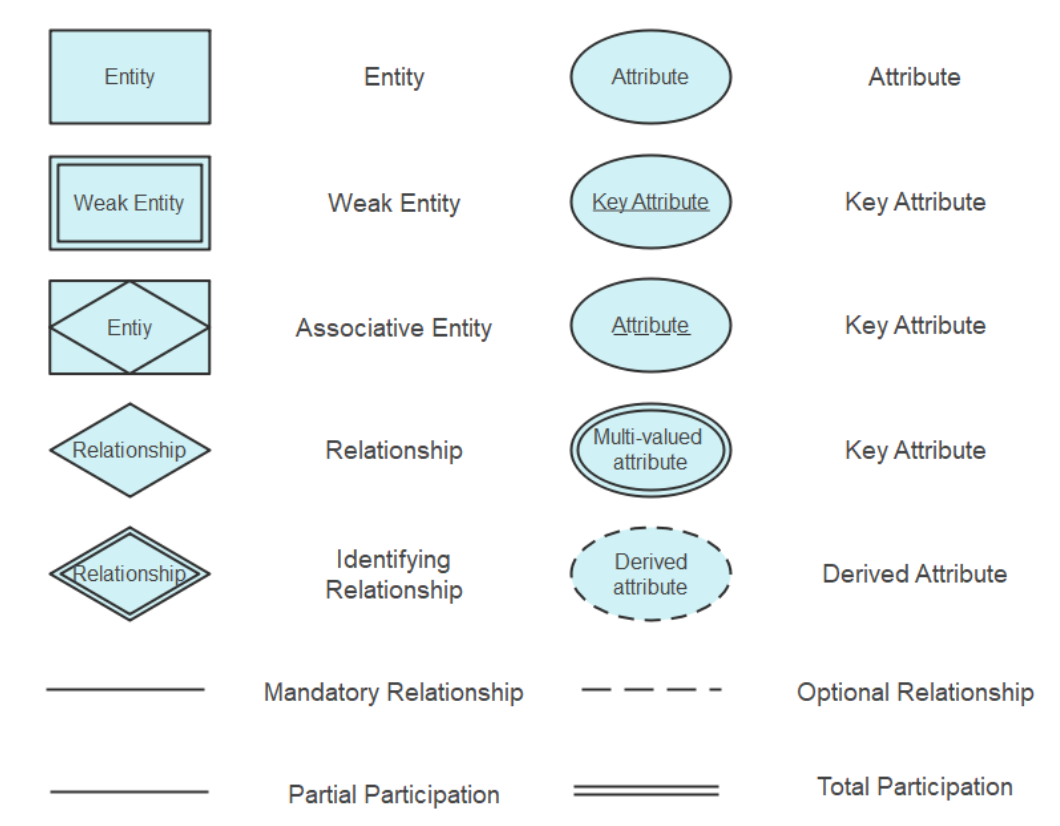
\includegraphics[width=5in]{dbms.png}
	\item \textbf{\textit{Procedure for Drawing ER Diagram:}} 
	\begin{itemize}
		\item Identify the Entities
		\item Draw relationship table
		\item Draw rough er diagram.
		\item Draw each entity in depth, that have all the attributes.
		\item Show the cardinality of each relationship.
	\end{itemize}
	\item \textbf{\textit{Entities in the Problem Statement:}}
	\begin{itemize}
		\item Student
		\item Course
		\item Course Offering
		\item instructor
	\end{itemize}
	\item \textbf{\textit{Relationships in the Problem Statement:}}
	\begin{itemize}
		\item Student Enrolled in Course Offering
		\item Course Offering taught by Instructor
		\item Course offering contains Course offering
	\end{itemize}
\end{enumerate}
\section{\textbf{Platform}}
Mac OS 64-bits
\section{\textbf{Output}}

\section{\textbf{Conclusion}}
In this assignment we have learned how to draw an ER diagram for a given problem statement. We have also learned about the different types of relationships and entities.
\section{\textbf{FAQ's}}
\begin{enumerate}
	\item What are different types of attributes?\\
	
	\begin{itemize}
		\item \textbf{Simple Attribute:} A simple attribute is an attribute that has only one value.
		\item \textbf{Composite Attribute:} A composite attribute is an attribute that has more than one value.
		\item \textbf{Multivalued Attribute:} A multivalued attribute is an attribute that has more than one value.
		\item \textbf{Derived Attribute:} A derived attribute is an attribute that is calculated from other attributes.
		\item \textbf{Composite Key:} A composite key is a primary key that consists of more than one attribute.
	\end{itemize}
	\item What do you mean by primary key and foreign key?
	
	\begin{itemize}
		\item \textbf{Primary Key:} A primary key is a unique identifier for each record in table. It is a unique identifier for an entity.
		\item \textbf{Foreign Key:} A foreign key is a field in a table that is a primary key in another table. It is a primary key of another entity.
	\end{itemize}
	\item What is weak entity?\\
	
	\textbf{Weak Entity:} A weak entity is an entity that cannot exist on its own. It must have a relationship with another entity. A weak entity is identified by a relationship with another entity. It must use a foreign key in conjunction with its attributes to create a primary key.\\
	
	\textbf{Example:} A Room can only exist in a Building. on the other hand, a Building can exist without a Room. Therefore, Room is a weak entity.
\end{enumerate}
\end{document}